
\begin{figure*}
	\centering
	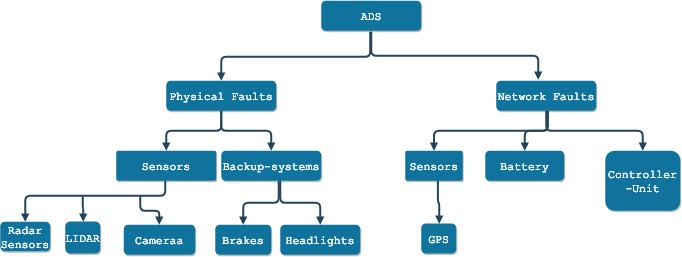
\includegraphics[width=0.8\linewidth]{Fault-modelgeneral}
	\caption[Fault-model for ADS]{This shows a general fault model of Autonomous Driving Systems. We have kept it generic enough to be considered for different Autonomous systems. However, our work is oriented towards autonomous cars.}
	\label{fig:fault-modelgeneral}
\end{figure*}
\section{Background} \label{background}
\subsection{ Autonomous Cars}
Self-driving autonomous cars use various technologies to provide an effortless mode of transportation. In order for autonomous cars to work effectively, proper synchronization of advanced sensors collecting data from surrounding environments and advanced algorithms processing this data in real time is necessary. The main components of a self-driving car are sensors, computer processors, actuators, batteries and back-up systems.

\subsection{Sensors}
Sensors are the core components in a self-driving car. We will talk about them in a little more detail since our research goal is to find error rate in self-driving cars caused by sensor faults. The core sensors of a self-driving car are as follows:

\smallskip
%Major sensors
\subsubsection{Radar sensors}
Radar sensors help autonomous vehicles in determining road dynamics such as detours, collisions and obstacles. Radar uses radio waves to determine the range, angle, or velocity of other objects present in the environment. Radar sensors are usually mounted on the bumper (two in the front and two in the back).

\smallskip
\subsubsection{Optics}
High powered cameras in conjunction with Radar sensors are another vital component of the autonomous vehicles. The camera setup on each car differs according to the manufacturer. The main goal of the camera placement is to get the surrounding views covered properly so that the processor can take correct decisions. Some manufacturers use a single camera on the windshield ~\cite{singlecamera} whereas some vehicles require multiple cameras placed equidistant from each other to get overlapped views. The processor can use the views to calculate the depth of the field and perform semantic segmentation of the captured images.

\smallskip
\subsubsection{GPS}
Global Positioning System sensor is very similar to the sensors we use for navigation maps on our mobile phones. However, GPS in autonomous vehicles is very important since we enter the destination point and the start point of our trip. The GPS works in conjunction with other sensors and Deep learning software ~\cite{GPS} in order to guide the vehicle in the correct direction to reach the destination.

\smallskip
\subsubsection{LIDAR}
Laser Illuminating Detection and Ranging (LIDAR) is used for creating 3D maps of the environment of an ADS. LIDAR unit resembles a spinning siren light and has a range of up to 100 meters. The goal of LIDAR is to provide driver-less cars with accurate long-range detection. LIDAR continuously performs 360-degree rotations in order to scan its surroundings. The sensor generates raw information about the world and the information is sent to the processor which digs out the relevant information in order to guide the vehicle and take decisions.

%\subsection{LIDAR}
%Since we are trying to determine the failure rates of LIDAR, we give a brief overview of how LIDAR units work in an autonomous car.
%
%%LiDAR working
%The autonomous car LIDAR units follow four steps in order to function:
%\begin{enumerate}
%	\item The LIDAR unit which is continuously rotating emits a laser beam generated by the laser emitter present inside LIDAR.
%	\item The laser bounces off the an object. The object is usually something solid and the moment, laser hits the first solid object it bounces off and returns to LIDAR.
%	\item The gathered light is then bounced downwards to the receiver, where the light is interpreted. 
%	\item This is a continuous process in all directions and the data gets sent to the processor which generates a map of its surroundings.
%\end{enumerate}

\subsection{Camera}
Cameras are one of the most important and expensive sensors in autonomous driving systems. The reason we chose Camera for our experimentation is because of the availability of test-beds in the form of CARLA. The fault-model for cameras has been described in Fig. 1. There are two categories of cameras used in Autonomous Driving systems.

\smallskip
\subsubsection{Rear and 360° Cameras} 
Rear and 360-degree cameras support the driver with a better representation of the environment outside the vehicle. Luxury class car makers now use such cameras to provide virtual, three-dimensional images of the surroundings of the car.

\smallskip
\subsubsection{Forward-Facing Camera Systems}
These camera systems are used for detection in medium to high range, i.e. area between 100 and 275 yards. These cameras use the algorithms to automatically detect objects, classify them, and determine the distance from them. For example, the cameras can identify pedestrians and cyclists, motor vehicles, side strips, bridge abutments, and road margins. The algorithms are also used to detect traffic signs and signals.


